\section{Управление рисками предприятия, методы оценки рисков}

Управление рисками --- это процессы, связанные с идентификацией, анализом рисков и принятием решений, которые включают максимизацию положительных и минимизацию отрицательных последствий наступления рисковых событий. Процесс управления рисками проекта обычно включает выполнение процедур, приведенных на рисунке \ref{fig:diagram-page-2}.

\begin{figure}[!h]
	\centering
	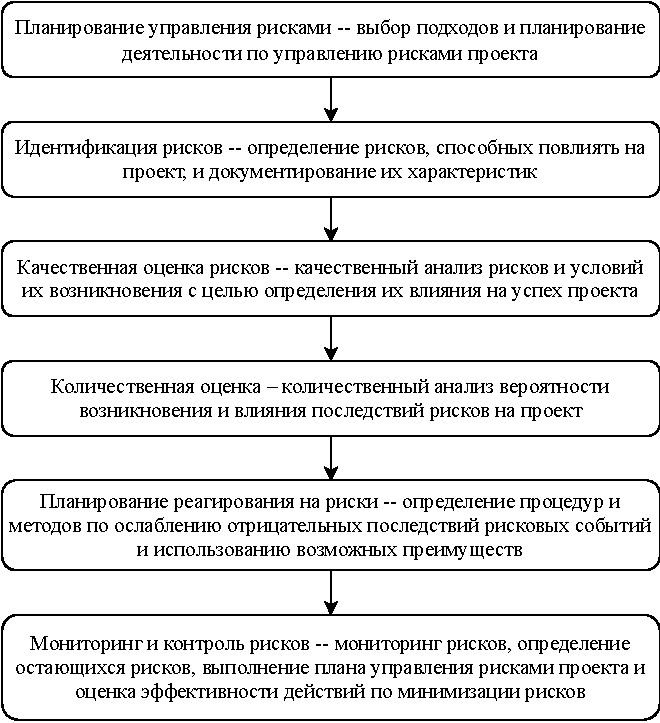
\includegraphics[width=0.7\linewidth]{Diagram-Page-2}
	\caption{Этапы управления рисками проекта}
	\label{fig:diagram-page-2}
\end{figure}

Планирование управления рисками --- процесс принятия решений по применению и планированию управления рисками для конкретного проекта. Этот процесс может включать в себя решения по организации, кадровому обеспечению процедур управления рисками проекта, выбор предпочтительной методологии, источников данных для идентификации риска, временной интервал для анализа ситуации. Важно спланировать управление рисками, адекватное как уровню и типу риска, так и важности проекта для организации.

Идентификация рисков --- заключается в систематическом выявлении рисков, характерных для определенного вида деятельности, и определении их характеристик.

Идентификация сводится к выявлению возможных проблем. 
Под «проблемой» понимают что-либо (событие, объект, человека, идею), что может встать между организацией и ее целями.
Необходимо определить, что пойдет «не так», чтобы затем решить, как это устранить или обойти.

Идентификация риска --- процесс нахождения, составления перечня и описания элементов риска.
Основные элементы риска:
\begin{itemize}
\item  причины, приводящие к наступлению опасного явления;
\item опасные явления (события), оказывающие воздействие на объект;
\item виды воздействия, которые могут привести к изменению состояния объекта;
\item последствия, представляющие собой потери из-за воздействия, и их оценку со стороны субъекта;
\item факторы риска, влияющие на вероятность реализации риска и тяжесть последствий.
\end{itemize}

Качественная оценка рисков – процесс представления качественного анализа идентификации рисков и определения рисков, требующих быстрого реагирования. Такая оценка рисков определяет степень важности риска и выбирает способ реагирования. Доступность сопровождающей информации помогает легче расставить приоритеты для разных категорий рисков. Качественная оценка рисков это оценка условий возникновения рисков и определение их воздействия на проект стандартными методами и средствами. Использование этих средств помогает частично избежать неопределенности, которые часто встречаются в проекте. В течение жизненного цикла проекта должна происходить
постоянная переоценка рисков.

Количественная оценка рисков определяет вероятность возникновения рисков и влияние последствий рисков на проект, что помогает группе управления проектами верно принимать решения и избегать неопределенностей. Количественная оценка рисков позволяет определять:
\begin{itemize}
\item вероятность достижения конечной цели проекта,
\item степень воздействия риска на проект и объемы непредвиденных затрат и материалов, которые могут понадобиться,
\item риски, требующие скорейшего реагирования и большего внимания, а также влияние их последствий на проект,
\item фактические затраты, предполагаемые сроки окончания.
\end{itemize}

Количественная оценка рисков часто сопровождает качественную оценку и также требует процесс идентификации рисков. Количественная и качественная оценка рисков могут использоваться по отдельности или вместе, в зависимости от располагаемого времени и бюджета, необходимости в количественной или качественной оценке рисков.

Планирование реагирования на риски --- это разработка методов и технологий снижения отрицательного воздействия рисков на проект. Берет на себя ответственность за эффективность защиты проекта от воздействия на него рисков. Планирование включает в себя идентификацию и распределение каждого риска по категориям. Эффективность разработки реагирования прямо определит, будут ли последствия воздействие риска на проект положительными или отрицательными. 

Стратегия планирования реагирования должна соответствовать типам рисков, рентабельности ресурсов и временным параметрам. Вопросы, обсуждаемые во время встреч, должны быть адекватны задачам на каждой стадии проекта, и согласованы со всеми членами группы по управлению проектом. Обычно требуются несколько вариантов стратегий реагирования на риски.

Мониторинг и контроль следят за идентификацией рисков, определяют остаточные риски, обеспечивают выполнение плана рисков и оценивают его эффективность с учетом понижения риска. Показатели рисков, связанные с осуществлением условий выполнения плана фиксируются. Мониторинг и контроль сопровождает процесс внедрения проекта в жизнь.

Качественный контроль выполнения проекта предоставляет информацию, помогающую принимать эффективные решения для предотвращения возникновений рисков. Для предоставления полной информации о выполнении проекта необходимо взаимодействие между всеми менеджерами проекта.

Целью мониторинга и контроля является выяснить, было ли:
\begin{itemize}
\item Система реагирования на риски внедрена в соответствии с планом
\item Реагирование достаточно эффективно или необходимы изменения
\item Риски изменились по сравнению с предыдущим значением
\item Наступление влияния рисков
\item Необходимые меры приняты
\item Воздействие рисков оказалось запланированным или явилось случайным результатом.
\end{itemize}

Контроль может повлечь за собой выбор альтернативных стратегий, принятие корректив, перепланировку проекта для достижения базового плана. Между менеджерами проекта и группой риска должно быть постоянное взаимодействие, должны фиксироваться все изменения и явления. Отчеты по выполнению проекта должны формироваться регулярно.





















